\subsection{System}
Ein System besteht aus mehreren Einzelgeräten, mit welchen, wie vorhin beschrieben, das Zählen, die Kategorisierung und die Geschwindigkeitsmessung durchgeführt wird. Es werden mehrere Geräte benötigt, um den Verkehrsfluss im definiert, begrenzten Gebiet darstellen zu können. Dabei konnte der Verkehrsfluss mithilfe des aufgenommenen Zeitstempels und der Fahrtrichtung statistisch rekonstruiert werden. Hierbei konnte das vorhin erstellte Netzwerk des begrenzten Gebietes als Darstellungsgrundlage verwendet werden. Zunächst wurden die nächstgelegenen Geräte, welche auf direktem Weg erreichbar sind, identifiziert und von diesen die Daten des Feature Vektors extrahiert. Diese Daten wurden dann nach dem Zeitstempel sortiert und mit einem Index versehen. Nachdem die Daten vorbereitet waren, wurde die voraussichtliche Durchfahrtszeit anhand der Abstände der Geräte anhand einer Testmessung bestimmt. Die höchste Wahrscheinlichkeit, welchen Weg der Verkehrsteilnehmer nahm, konnte aufgrund dessen berechnet und anschliessened eingezeichnet werden. Der geschilderte Vorgang konnte mit jedem Geräte durchgeführt und diese untereinander verglichen werden. Die möglichen Wege wurden dem Netzwerk ergänzt und somit konnte die folgende Auswertung (\fref{bAuswertung}) durchgeführt werden. 

\begin{figure}[H]
  \centering
  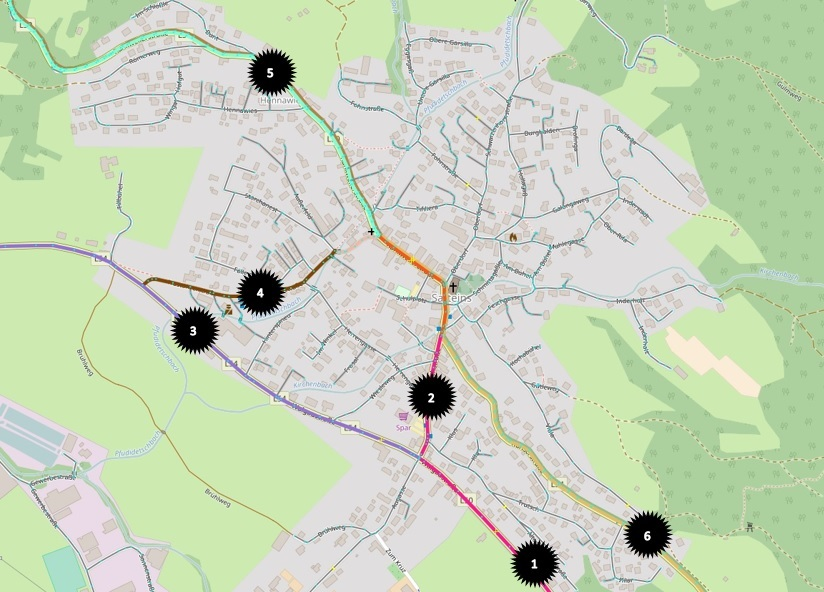
\includegraphics[width=0.6\textwidth]{Resultate/Auswertung.jpg} 
  \caption{Darstellung des Verkehrsflusses in Satteins.}
  \label{bAuswertung}
\end{figure}
In \tref{tVerkehrsfluss} ist der Verkehrsfluss von jedem Gerät zu seinem direkten Nachfolger tabellarisch dargestellt. 

\setlength\tabcolsep{5pt}

\begin{table}[H]
\centering
\begin{tabular}{|p{1.5cm}|p{1.5cm}|p{1.5cm}|p{1.5cm}|p{1.5cm}|p{1.5cm}|p{1.5cm}|p{1.5cm}|}
\hline
	von/nach & 1 & 2 & 3 & 4 & 5 & 6 & Out \\ \hline
	1 &  & 952 & 949 &  &  &  & 1703 \\ \hline
	2 & 326 & 0 & 279 & 105 & 434 & 275 & 0 \\ \hline
	3 & 996 & 0 &  &  &  &  & 1468 \\ \hline
	4 &  & 149 &  &  & 105 & 84 & 520 \\ \hline
	5 &  & 723 &  & 159 & 521 & 224 & 1668 \\ \hline
	6 &  & 313 &  & 78 & 426 &  & 327 \\ \hline
\end{tabular}
\caption{Tabelarische Darstellung des Verkehrsflusses.}
\label{tVerkehrsfluss}
\end{table}

\setlength\tabcolsep{0pt}